\documentclass[tikz,border=1.5mm]{standalone}

\usepackage{amsmath}
\usetikzlibrary{arrows.meta,positioning,fit,backgrounds}

\definecolor{figdark}{gray}{0.25}
\definecolor{figmid}{gray}{0.55}
\definecolor{figlight}{gray}{0.90}
\definecolor{figstate}{gray}{0.78}

\begin{document}
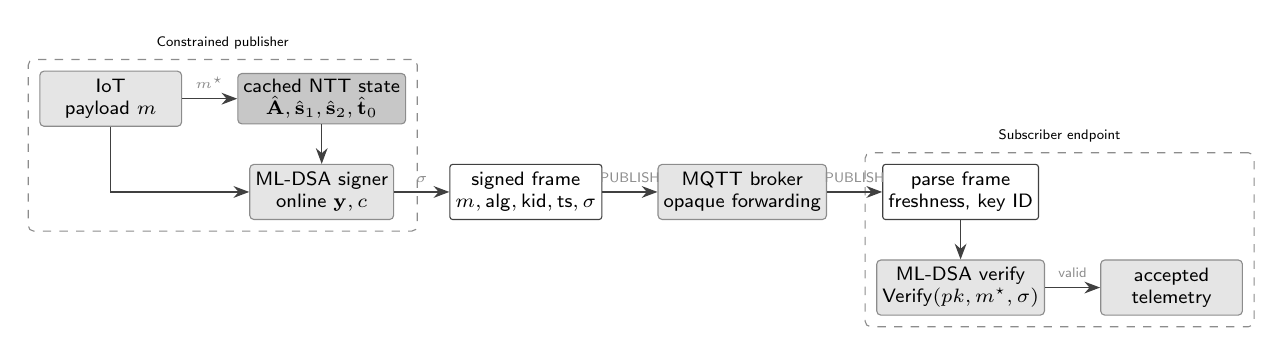
\begin{tikzpicture}[
    font=\scriptsize\sffamily,
    node distance=5mm and 7mm,
    block/.style={rectangle, draw=figmid, fill=figlight, rounded corners=1.5pt,
        align=center, minimum width=18mm, minimum height=7mm, inner sep=2pt},
    state/.style={rectangle, draw=figmid, fill=figstate, rounded corners=1.5pt,
        align=center, minimum width=20mm, minimum height=6mm, inner sep=2pt},
    frame/.style={rectangle, draw=figdark, fill=white, rounded corners=1pt,
        align=center, minimum width=19mm, minimum height=7mm, inner sep=2pt},
    group/.style={draw=figmid, dashed, rounded corners=2pt, inner sep=4pt},
    arrow/.style={-{Stealth[length=2mm]}, draw=figdark, line width=0.45pt},
    note/.style={font=\tiny\sffamily, align=center, text=figmid}
]
    \node[block] (sensor) {IoT\\payload $m$};
    \node[state, right=of sensor] (cache) {cached NTT state\\$\hat{\mathbf{A}},\hat{\mathbf{s}}_1,\hat{\mathbf{s}}_2,\hat{\mathbf{t}}_0$};
    \node[block, below=of cache] (sign) {ML-DSA signer\\online $\mathbf{y},c$};
    \node[frame, right=of sign] (payload) {signed frame\\$m,\mathsf{alg},\mathsf{kid},\mathsf{ts},\sigma$};
    \node[block, right=of payload] (broker) {MQTT broker\\opaque forwarding};
    \node[frame, right=of broker] (parse) {parse frame\\freshness, key ID};
    \node[block, below=of parse] (verify) {ML-DSA verify\\$\mathsf{Verify}(pk,m^\star,\sigma)$};
    \node[block, right=of verify] (accept) {accepted\\telemetry};

    \draw[arrow] (sensor) -- node[above, note] {$m^\star$} (cache);
    \draw[arrow] (cache) -- (sign);
    \draw[arrow] (sensor.south) |- (sign.west);
    \draw[arrow] (sign) -- node[above, note] {$\sigma$} (payload);
    \draw[arrow] (payload) -- node[above, note] {PUBLISH} (broker);
    \draw[arrow] (broker) -- node[above, note] {PUBLISH} (parse);
    \draw[arrow] (parse) -- (verify);
    \draw[arrow] (verify) -- node[above, note] {valid} (accept);

    \begin{scope}[on background layer]
        \node[group, fit=(sensor)(cache)(sign), label={[font=\tiny\sffamily]above:Constrained publisher}] {};
        \node[group, fit=(parse)(verify)(accept), label={[font=\tiny\sffamily]above:Subscriber endpoint}] {};
    \end{scope}
\end{tikzpicture}
\end{document}
